\documentclass[../../../patent_v1.tex]{subfiles}

\begin{document}

\subsection{Depth estimation unit}

\subsubsection{Web Cam}

(LAPCARE LAPCAM)

\begin{figure}[ht]
    \centering
    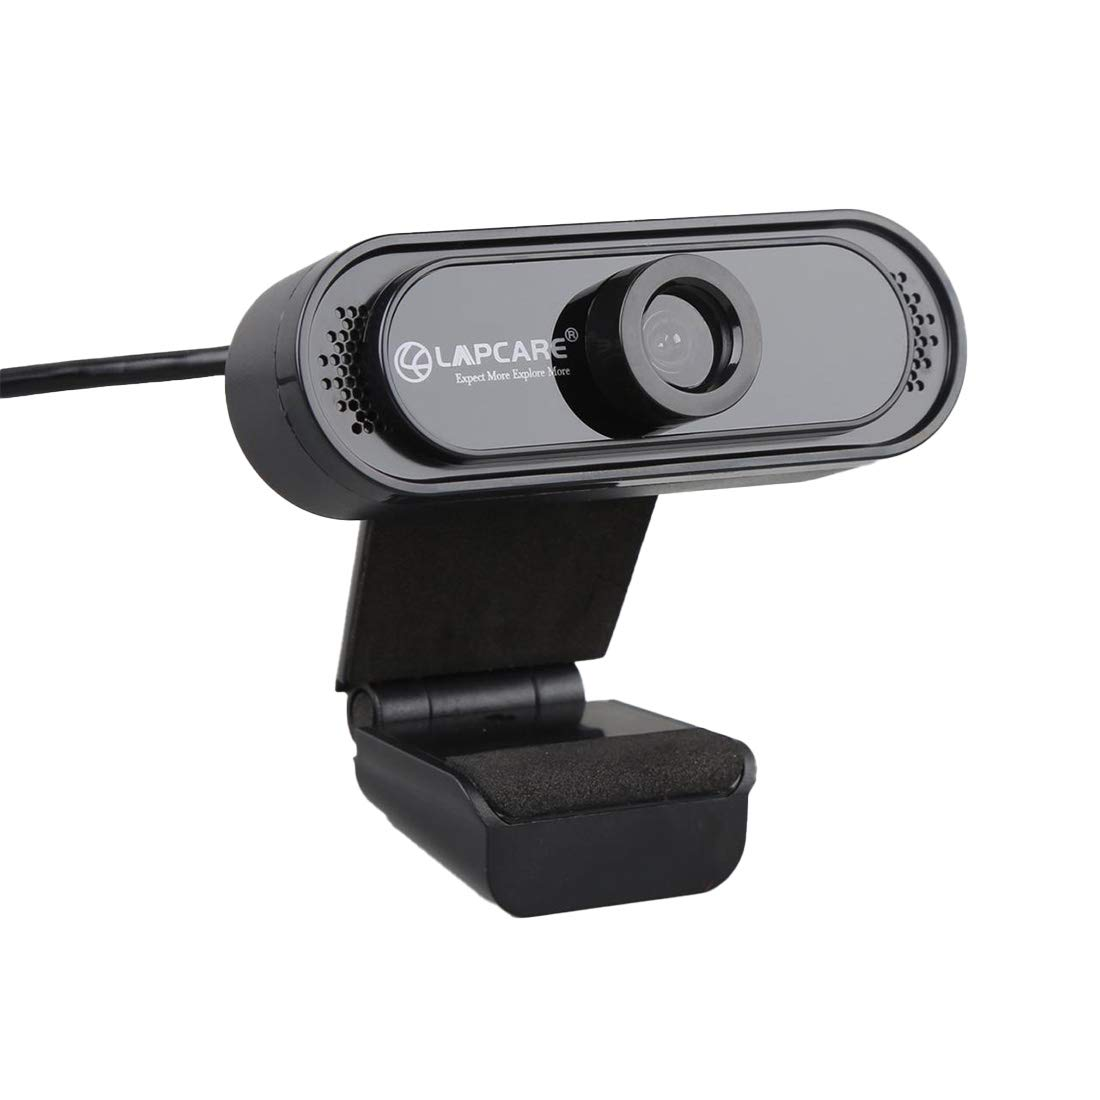
\includegraphics[width=4cm]{web_cam.jpg}
    \caption{Web cam}
\end{figure}

\FloatBarrier

\begin{description}
    \item[1.]1280 x 720 pixels @ 720p resolution
    \item[2.]Automatic low light correction
    \item[3.]Plug and play Linux compatible, High-Speed USB 2.0   
\end{description}


\subsection{Microprocessor}

Microprocessor serves an important role in DAC application, data processing estimation 
and controlling the response hardware in real time.

\begin{figure}[ht]
    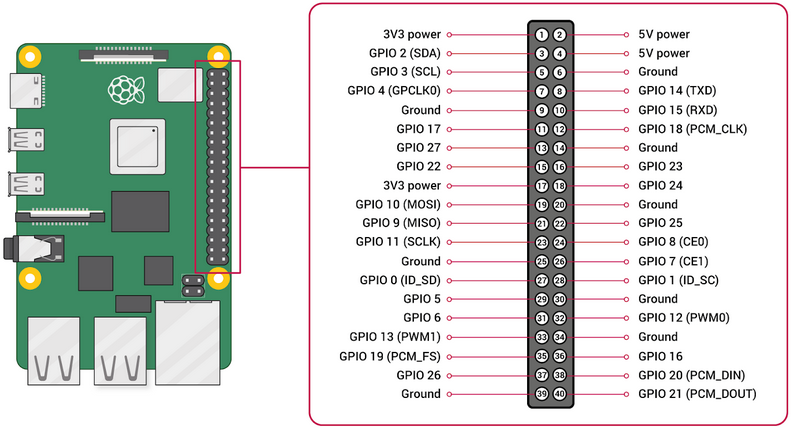
\includegraphics[width=\columnwidth]{raspberry_pi.png}
    \caption{Microprocessor (Raspberry Pi 4B 4GB)}
\end{figure}

\FloatBarrier

Raspberry Pi 4B 4GB RAM model comes packed with, 

\begin{description}
    \item[1.]Quad core Cortex-A72 64-bit @ 1.5 GHz clock and uses ARM v8 architecture, 
    with 4GB LPDDR4-3200 SDRAM.
    \item[2.]2.4 and 5 GHz IEEE 802.11ac wireless wifi hardware.
    \item[3.]2 Micro HDMI ports.
    \item[4.]H.265 (4kp60 decode), H264 (1080p60 decode, 1080p30 encode).
    \item[5.]OpenGL ES 3.0 graphics.
    \item[6.]Micro-SD card slot for loading operating system and data storage.
    \item[7.]4 USB ports.
    \item[8.]Software PWM on all pins and Hardware on GPIO12, GPIO13, GPIO18, GPIO19.
    \item[9.]SPI
    \begin{description}
        \item[-]SPI0 : MOSI (GPIO10), MISO (GPIO09), SCLK (GPIO11), CE0 (GPIO08), CE1 (GPIO07)
        \item[-]SPI1 : MOSI (GPIO20), MISO (GPIO19), SCLK (GPIO21), CE0 (GPIO18), CE1 (GPIO17), CE2 (GPIO16).  
    \end{description}  
\end{description}

\subsection{Mechanical unit}

\subsubsection{Servo Motors}

(SG90 Servo)

\begin{figure}[ht]
    \centering
    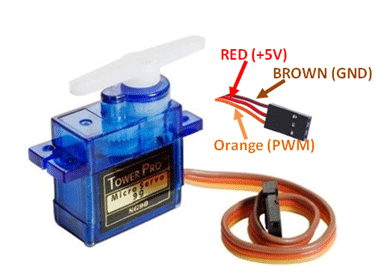
\includegraphics[width=5cm]{servo.png}
    \caption{SG90 Servo}
\end{figure}

\FloatBarrier

\begin{description}
    \item[1.]180\si{\degree} rotation (90\si{\degree} in each direction).
    \item[2.]Torque 2.5 kg-cm
    \item[3.]Voltage 4.8-6 V  
    \item[4.]Speed 0.12 sec/60\si{\degree}
\end{description}

\subsection{Audio processor unit}

\subsubsection{Audio Amplifier}

(LM386N-1)

\begin{figure}[ht]
    \centering
    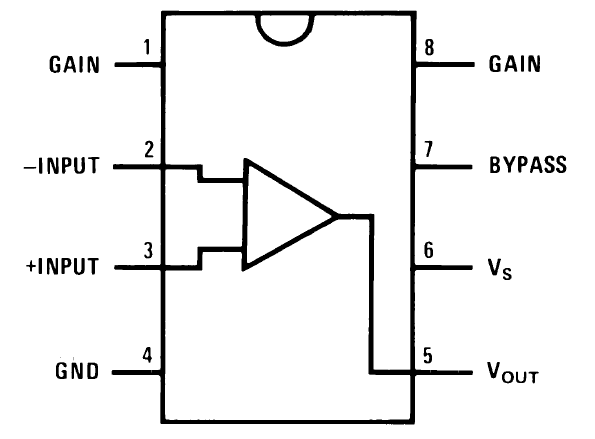
\includegraphics[width=5cm]{lm386.png}
    \caption{LM386N-1 pin-out}
\end{figure}

\FloatBarrier

\begin{description}
    \item[1.]Operating Supply Voltage (Vs) 4 - 12 V
    \item[2.]Voltage gain 20 - 200
    \item[3.]Output power 325 mW
\end{description}

\subsubsection{Digital Potentiometer}

(MCP42010)

\begin{figure}[ht]
    \centering
    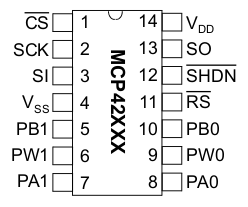
\includegraphics[width=5cm]{mcp42010.png}
    \caption{MCP42010 pin-out}
\end{figure}

\FloatBarrier

\begin{description}
    \item[1.]Potentiometer values 10 k\si{\ohm}
    \item[2.]256 taps for each potentiometer
    \item[3.]2 channel
    \item[4.]SPI serial interface (mode 0, 0 and 1, 1)
    \item[5.]Single power operation (2.7V - 5.5V)
    \item[6.]Industrial temperature range: -40\si{\celsius} to +85\si{\celsius} 
    \item[7.]External temperature range: -40\si{\celsius} to +125\si{\celsius}    
\end{description}
 
\subsection{Speakers}

The final component is the speakers, which are mounted on servos and the sound is 
dynamically controlled using Audio Processor. They have mounted on four corners of the 
room to form a four-channel audio system. 

For this application, we are using 4\si{\ohm} speakers to deliver four-channel output.

\end{document}